%-------------------------------------------------------------------------------
% 请勿删除本注释
% Free Response Question 2
%
% 指引:
% 如在小问之前有通用问题描述,请放置于此
%-------------------------------------------------------------------------------
\begin{figure}[h]
\centering
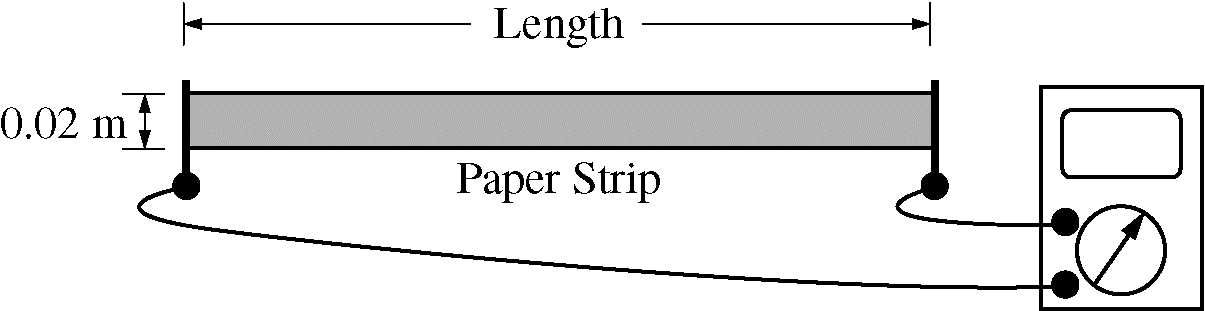
\includegraphics[scale=0.3]{images/img-016-029.png}
\end{figure}


\question
A physics student wishes to measure the resistivity of slightly conductive paper that has a thickness of $1.0 \times 10^{-4} \mathrm{~m}$. The student cuts a sheet of the conductive paper into strips of width $0.02 \mathrm{~m}$ and varying lengths, making five resistors labeled R1 to R5. Using an ohmmeter, the student measures the resistance of each strip, as shown above. The data are recorded below.


\begin{table}[h]
\centering
\begin{tabular}{|c|c|c|c|c|c|}
\hline Resistor & $\mathrm{R} 1$ & $\mathrm{R} 2$ & $\mathrm{R} 3$ & $\mathrm{R} 4$ & $\mathrm{R} 5$ \\
\hline Length $(\mathrm{m})$ & $0.020$ & $0.040$ & $0.060$ & $0.080$ & $0.100$ \\
\hline Resistance $(\Omega)$ & 80,000 & 180,000 & 260,000 & 370,000 & 440,000 \\
\hline
\end{tabular}
\end{table}


% 请删除并替换本行,与上一行 \question 之间不要留空行

\begin{parts}

%-------------------------------------------------------------------------------
% 请勿删除本注释
% Part (a)
%
% 指引:
% 如在小问之前有通用问题描述,请放置于此
%-------------------------------------------------------------------------------

\part
Use the grid below to plot a linear graph of the data points from which the resistivity of the paper can be determined. Include labels and scales for both axes. Draw the straight line that best represents the data. % 请删除并替换本行,与上一行 \part 之间不要留空行

\begin{figure}[H]
\centering

\includegraphics[scale=0.2]{images/img-016-030.png}
\end{figure}


%-------------------------------------------------------------------------------
% 请勿删除本注释
% Part (b)
%
% 指引:
% 如在小问之前有通用问题描述,请放置于此
%-------------------------------------------------------------------------------

\part
Using the graph, calculate the resistivity of the paper. % 请删除并替换本行,与上一行 \part 之间不要留空行

\begin{figure}[H]
\centering
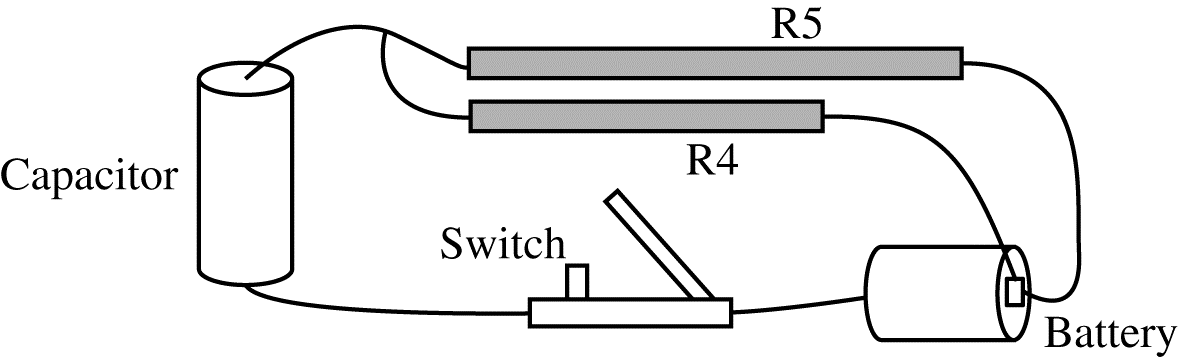
\includegraphics[scale=0.3]{images/img-017-031.png}
\end{figure}

The student uses resistors R4 and R5 to build a circuit using wire, a $1.5 \mathrm{~V}$ battery, an uncharged $10 \mu \mathrm{F}$ capacitor, and an open switch, as shown above.


%-------------------------------------------------------------------------------
% 请勿删除本注释
% Part (c)
%
% 指引:
% 如在小问之前有通用问题描述,请放置于此
%-------------------------------------------------------------------------------

\part
Calculate the time constant of the circuit. % 请删除并替换本行,与上一行 \part 之间不要留空行

%-------------------------------------------------------------------------------
% 请勿删除本注释
% Part (d)
%
% 指引:
% 如在小问之前有通用问题描述,请放置于此
%-------------------------------------------------------------------------------

\part
At time $t=0$, the student closes the switch. On the axes below, sketch the magnitude of the voltage $V_{c}$ across the capacitor and the magnitudes of the voltages $V_{\mathrm{R} 4}$ and $V_{\mathrm{R} 5}$ across each resistor as functions of time $t$. Clearly label each curve according to the circuit element it represents. On the axes, explicitly label any intercepts, asymptotes, maxima, or minima with values or expressions, as appropriate. % 请删除并替换本行,与上一行 \part 之间不要留空行

\begin{figure}[h]
\centering
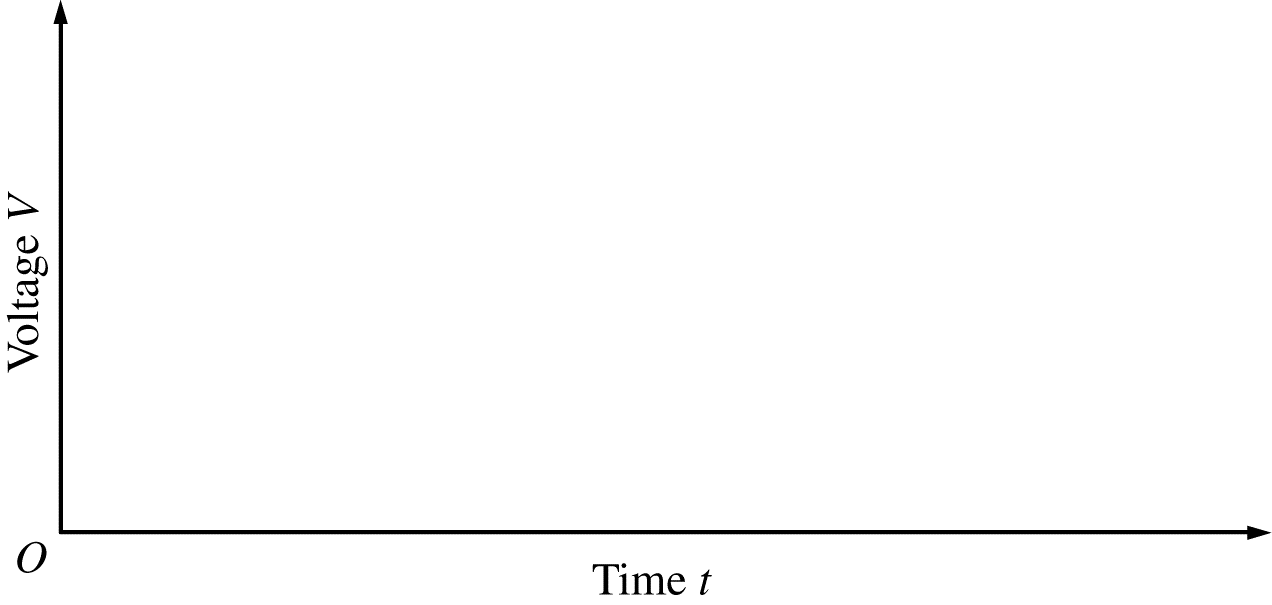
\includegraphics[scale=0.3]{images/img-017-032.png}
\end{figure}


\end{parts}
